\documentclass[12pt,brazil,a4paper]{article}
\usepackage[T1]{fontenc}
\usepackage[utf8]{inputenc}
\usepackage{geometry}
\usepackage{booktabs}
\usepackage{graphicx}
\usepackage{listings}
\usepackage{latexsym}
\usepackage{hyperref}
\usepackage{amsmath}
\usepackage{pgfplots}
\pgfplotsset{compat=1.17}
\usepackage{float}
\geometry{verbose,tmargin=2cm,bmargin=2cm,lmargin=2cm,rmargin=2cm}
\RequirePackage{times}
\usepackage{babel}

\setlength{\jot}{0.25\jot}

\begin{document}

\title{O Jantar dos Filósofos}

\author{Douglas Lisboa Silvano\thanks{\texttt{douglas.silvano@edu.pucrs.br}}, Luiza Militão Pereira\thanks{\texttt{l.militao@edu.pucrs.br}}, Renan Bertoletti Araujo\thanks{\texttt{renan.bertoletti@edu.pucrs.br}}\\
Escola Politécnica — PUCRS}

\date{\today}
\maketitle

%% ------------------------------------------------------------------
\begin{abstract}
Comparamos quatro implementações em Go do jantar dos filósofos: sequencial (V0), concorrente com \textit{deadlock} (V1), com garçom/semáforo (V2) e com ordenação global de garfos (V3). Cada filósofo executou 20 ciclos (pensar 20~ms, comer 30~ms), com 5 execuções por versão. A V1 travou em 12 de 20 execuções, com espera circular entre os cinco filósofos. A V0 levou 5,19~s; a V2 com limite 1 levou 3,12~s (comer serializado); a V3 levou 1,65~s, com até dois filósofos comendo ao mesmo tempo. O tempo total acompanha o grau de concorrência, e mais sincronização não significou melhor desempenho.

\end{abstract}

%% ------------------------------------------------------------------
\section{Introdução}
% Problema dos filósofos jantando (Dijkstra), objetivo do trabalho e organização do relatório.
Proposto por \textit{{Edsger Dijkstra}}, o problema do jantar dos filósofos é um clássico dilema utilizado para o estudo de sincronização e concorrência em programas.

Neste jantar, cinco filósofos estão sentados em uma mesa redonda, e entre cada par de filósofos existe um único garfo. Cada filósofo alterna entre dois estados: pensando e comendo. Para comer, o filósofo precisa utilizar simultaneamente os dois garfos ao seu lado - o da direita e da esquerda. E quando ele termina de comer, começa a pensar.

O objetivo do trabalho é encontrar uma solução, através de um programa concorrente, para gerenciar o acesso aos garfos compartilhados sem causar falhas graves no sistema, como \textit{{deadlocks}} ou \textit{{starvation}}.

Através de quatro diferentes versões, comparamos diferentes estratégias para o problema apresentado, e neste relatório apresentamos a melhor solução encontradas e as razões por trás dessa decisão.

%% ------------------------------------------------------------------
\section{Implementações}
Dentre nossas 4 implementações, todas mantém uma estrutura base: usam 5 filósofos, 20 ciclos, 20 ms para pensar e 30 ms para comer, e o mesmo bloco de estatísticas. Os garfos seguem a figura trazida no enunciado do trabalho: o filósofo P$i$ ($i=1,\dots,5$) usa à esquerda o garfo F$(i-1)$, sendo F5 no caso de P1, e à direita o garfo F$i$. Então P1 usa F5 e F1, P2 usa F1 e F2, e assim por diante até P5, que usa F4 e F5.

A espera medida é o tempo entre terminar de pensar e já ter os dois garfos. O máximo de filósofos comendo juntos vem de um contador atômico incrementado ao começar a comer e decrementado ao terminar.

\subsection{V0 -- Versão Sequencial}
Não há concorrência nessa versão: dois laços aninhados percorrem os ciclos $c=1..20$ e, dentro de cada ciclo, os filósofos P1 a P5. Cada chamada pensa, adquire, come e libera antes que o próximo filósofo comece. Como só um filósofo está ativo por vez, os garfos estão sempre livres.

Nessa versão, não há nenhum mecanismo de sincronização. Pensar e comer são simulados com \texttt{time.Sleep}. A espera é medida entre dois \texttt{time.Now()} consecutivos, sem operação no meio, e por isso é praticamente zero. O tempo total é medido com \texttt{time.Since}. O tempo esperado é $20\times5\times(20+30)\,\text{ms}=5$~s, e o programa imprime esse valor teórico ao final.

\begin{lstlisting}
for c := 1; c <= cfg.ciclos; c++ {
    for j := 0; j < cfg.n; j++ {
        filosofo(j, c)   // pensar, "adquirir", comer
    }
}
\end{lstlisting}

\subsection{V1 -- Versão Concorrente Sujeita a Deadlock}
Nessa evolução, cada filósofo é uma goroutine. No ciclo ele pensa, pega o garfo esquerdo, pausa um instante, pega o direito, come e então solta o direito e depois o esquerdo. Não existe ordem global entre os garfos.

Para sincronização, foi definido que cada garfo é um \texttt{sync.Mutex}, que garante exclusão mútua: um dono por vez. Nenhum outro mecanismo é usado.

Baseada em ``Five Forks and a Deadlock'' (R.~Alam). Para tornar o deadlock demonstrável, ajustamos o código base:

\begin{itemize}
\item A pausa entre pegar o 1º e o 2º garfo virou a flag \texttt{-atraso} (padrão 10~ms), o que aumenta a janela em que todos podem estar com um garfo na mão;
\item O tempo de pensar é sorteado entre 10 e 30~ms (\texttt{-jitter} 20~ms, média igual à das outras versões), então o deadlock deixa de ser certo. Com \texttt{-jitter 0} todos acordam juntos e o deadlock é certo já no ciclo 1;
\item Um ``vigia'' declara deadlock quando ninguém progride por 2~s. Progresso é pegar o primeiro garfo, começar a comer ou terminar de comer. Ao declarar, ele imprime a evidência: quem segura qual garfo, por qual espera, com quem está esse garfo e o ciclo de espera. Depois o runtime do Go aborta com \texttt{all goroutines are asleep - deadlock!}.
\end{itemize}

\begin{lstlisting}
f.pegar(f.esq)           // Lock no garfo esquerdo
time.Sleep(atraso)       // alarga a janela do deadlock
f.pegar(f.dir)           // Lock no garfo direito
// ... come ...
f.dir.Unlock(); f.esq.Unlock()
\end{lstlisting}

Como o \texttt{-atraso} entra na espera e o pensar é sorteado, as execuções da V1 que completam não são diretamente comparáveis com V0, V2 e V3. Por isso a V1 aparece na tabela separada por uma linha, só com as execuções concluídas.

\subsection{V2 -- Sem Deadlock, com Sincronização Excessiva}
Nessa tentativa de melhorar a versão anterior, a V1, um ``garçom'' limita quantos filósofos podem tentar pegar garfos ao mesmo tempo. O filósofo pensa, pede permissão ao garçom, pega o garfo esquerdo e depois o direito, come, solta os dois garfos e devolve a permissão. A permissão só volta depois de comer. Com limite menor que $N$ não há deadlock. No padrão (\texttt{-limite 1}), só um filósofo por vez adquire, come e libera, o que serializa o comer e é a sincronização excessiva pedida para esta versão. Também testamos limites 2 e 4 para ver o efeito do grau de concorrência.

Como mecanismos de sincronização, usa um semáforo contador, o garçom, e mais um \texttt{sync.Mutex} por garfo. Baseada em ``The Waiter Solution'' (R.~Alam). Go não tem semáforo nativo, então ele é um canal com buffer de capacidade igual ao limite. Enviar no canal é \texttt{pedir} e bloqueia se o buffer está cheio. Receber é \texttt{liberar}. O programa recusa limites fora de 1 a $N-1$.

\begin{lstlisting}
type garcom struct{ vagas chan struct{} }
func novoGarcom(limite int) *garcom {
    return &garcom{vagas: make(chan struct{}, limite)}
}
func (g *garcom) pedir()   { g.vagas <- struct{}{} } // bloqueia se cheio
func (g *garcom) liberar() { <-g.vagas }
\end{lstlisting}

\subsection{V3 -- Versão Concorrente Aprimorada}
Na versão final, todo filósofo pega primeiro o garfo de menor número e depois o de maior número, e solta na ordem inversa. É a hierarquia de recursos de Dijkstra. Não há coordenador central nem semáforo. Com a numeração da figura, só P1 (garfos F5 e F1) inverte a ordem esquerdo/direito: pega F1 e depois F5. Os demais pegam a esquerda e depois a direita. Isso equivale à solução assimétrica.

Para sincronização, apenas um \texttt{sync.Mutex} por garfo e uma ordem global de aquisição.

Com a implementação baseada em ``Global Resource Ordering'' (R.~Alam), cada garfo tem um \texttt{id}, e cada goroutine decide uma vez qual é o primeiro e qual é o segundo.

\begin{lstlisting}
primeiro, segundo := esq, dir
if dir.id < esq.id {
    primeiro, segundo = dir, esq
}
primeiro.Lock()
segundo.Lock()
// ... come ...
segundo.Unlock()
primeiro.Unlock()
\end{lstlisting}

\subsection{Análise Comparativa das Soluções}
\begin{center}
\small
\begin{tabular}{p{2.3cm}p{3.2cm}p{3.2cm}p{3.6cm}p{3cm}}
\toprule
 & V0 & V1 & V2 & V3\\
\midrule
Mecanismo de Sincronização & nenhum & \texttt{Mutex} por garfo & semáforo (canal) + \texttt{Mutex} & \texttt{Mutex} + ordem global\\
Deadlock & impossível & possível & impossível & impossível\\
Máx.\ comendo (teórico) & 1 & 2 & 1 (limite 1); 2 nos demais & 2\\
Ponto fraco & sem paralelismo & trava & serializa com limite 1 & sem garantia de justiça\\
\bottomrule
\end{tabular}
\end{center}
Com 5 garfos e 2 garfos por filósofo, no máximo 2 filósofos comem ao mesmo tempo, em qualquer versão. A V3 pode chegar a esse máximo sem coordenação central. A V2 com limite 1 não pode, e com limite 2 ou 4 só chega se os filósofos que comem simultaneamente não forem vizinhos.

%% ------------------------------------------------------------------
\section{Metodologia do Experimento}
Cada filósofo executa 20 ciclos de pensar $\rightarrow$ adquirir recursos $\rightarrow$ comer $\rightarrow$ liberar recursos. Todas as versões usam os mesmos tempos simulados (20~ms pensando e 30~ms comendo). Cada versão que conclui normalmente foi executada 5 vezes (V0, V2 com limites 1, 2 e 4, e V3), com a saída gráfica T/E desligada (\texttt{-q}) para não interferir no tempo. A V1 foi executada 20 vezes, porque o deadlock é probabilístico. Contamos quantas travaram e guardamos a primeira evidência.

Métricas coletadas: tempo total de execução, tempo médio de espera pelos garfos, maior tempo de espera observado, número máximo de filósofos comendo simultaneamente e ciclos concluídos por filósofo. A espera inclui, na V2, a espera pela permissão do garçom. O tempo é medido com \texttt{time.Now()} e \texttt{time.Since()}, e as estatísticas usam contadores atômicos. O script \texttt{run\_all.sh} executa tudo e calcula média e desvio padrão do tempo total.

\subsection{Ambiente de Execução}
\begin{itemize}
\item \textbf{Linguagem:} Go 1.26.6 (\texttt{darwin/arm64});
\item \textbf{Sistema operacional:} macOS (Darwin 25.6.0, arm64);
\item \textbf{Processador:} Apple M5, 10 cores lógicos disponíveis;
\item \textbf{Compilação:} \texttt{go build -o bin/v0 ./v0\_sequencial} (idem \texttt{v1\_deadlock}, \texttt{v2\_semaforo}, \texttt{v3\_ordenacao});
\item \textbf{Execução:} \texttt{./bin/v0 -q}, \texttt{./bin/v2 -limite 1 -q} (também 2 e 4), \texttt{./bin/v3 -q} e \texttt{./bin/v1}. Tudo foi automatizado por \texttt{bash run\_all.sh}.
\end{itemize}

%% ------------------------------------------------------------------
\section{Resultados}

\subsection{Tabela Comparativa}
\begin{table}[h]
\centering
\small
\begin{tabular}{lrrrr}
\toprule
Versão & Tempo total (s), média $\pm$ dp & Espera média (ms) & Maior espera (ms) & Máx.\ comendo\\
\midrule
V0 & 5,194 $\pm$ 0,005 & 0,000 & 0,003 & 1\\
V2 (limite 1) & 3,115 $\pm$ 0,003 & 100,799 & 124,099 & 1\\
V2 (limite 2) & 1,736 $\pm$ 0,048 & 32,410 & 93,010 & 2\\
V2 (limite 4) & 1,876 $\pm$ 0,694 & 40,344 & 124,136 & 2\\
V3 & 1,648 $\pm$ 0,068 & 25,150 & 124,136 & 2\\
\midrule
V1$^*$ (8 de 20) & 2,911 $\pm$ 0,545 & 91,7 & 122,1 & 2\\
\bottomrule
\end{tabular}
\caption{Média de 5 execuções por versão (tempo total com desvio padrão; espera média = média das médias; maior espera e máx.\ comendo = maior valor entre as 5 execuções). Em todas as execuções concluídas, todos os filósofos fizeram os 20 ciclos. $^*$A V1 só entra com as 8 de 20 execuções que não travaram; as outras 12 são analisadas na Seção~\ref{sec:v1}. Como o deadlock é probabilístico, essa linha é um subconjunto das execuções e não é comparável diretamente às demais (a V1 também usa uma pausa de 10~ms entre os garfos e pensar sorteado entre 10 e 30~ms). O desvio alto da V2 (limite 4) vem de uma execução de 3,12~s entre cinco de cerca de 1,56~s (Seção~\ref{sec:comboio}).}
\end{table}

\subsection{Gráficos}
\begin{figure}[H]
\centering
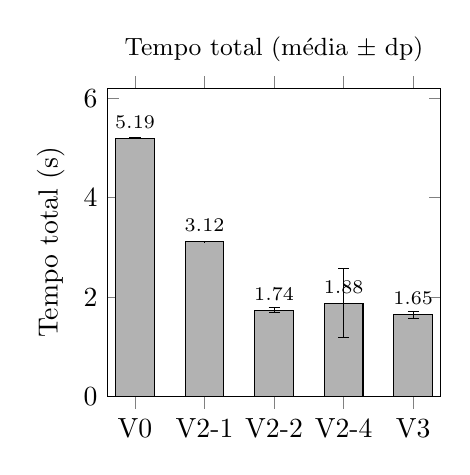
\begin{tikzpicture}
\begin{axis}[ybar, width=0.48\textwidth, height=5.5cm, bar width=14pt, ylabel={Tempo total (s)}, symbolic x coords={V0,V2-1,V2-2,V2-4,V3}, xtick=data, ymin=0, ymax=6.2, nodes near coords, nodes near coords style={font=\scriptsize,/pgf/number format/.cd,fixed,precision=2}, error bars/y dir=both, error bars/y explicit, title={Tempo total (média $\pm$ dp)}, title style={font=\small}]
\addplot[fill=gray!60] coordinates {(V0,5.194) +- (0,0.005) (V2-1,3.115) +- (0,0.003) (V2-2,1.736) +- (0,0.048) (V2-4,1.876) +- (0,0.694) (V3,1.648) +- (0,0.068)};
\end{axis}
\end{tikzpicture}
\hfill
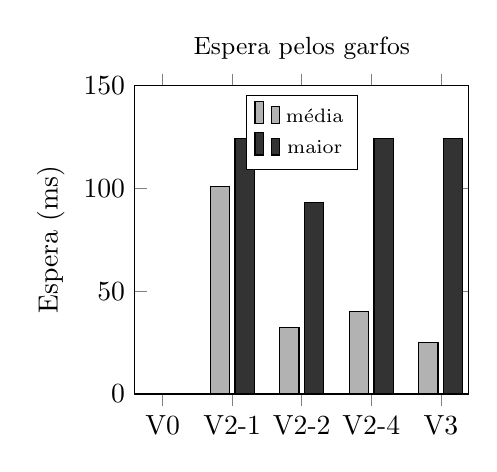
\begin{tikzpicture}
\begin{axis}[ybar, width=0.48\textwidth, height=5.5cm, bar width=7pt, ylabel={Espera (ms)}, symbolic x coords={V0,V2-1,V2-2,V2-4,V3}, xtick=data, ymin=0, ymax=150, legend style={font=\scriptsize, at={(0.5,0.97)}, anchor=north}, title={Espera pelos garfos}, title style={font=\small}]
\addplot[fill=gray!60] coordinates {(V0,0.0) (V2-1,100.8) (V2-2,32.4) (V2-4,40.3) (V3,25.2)};
\addplot[fill=black!80] coordinates {(V0,0.003) (V2-1,124.1) (V2-2,93.0) (V2-4,124.1) (V3,124.1)};
\legend{média, maior}
\end{axis}
\end{tikzpicture}
\caption{Tempo total e tempo de espera por versão (5 execuções cada).}
\end{figure}

\begin{figure}[H]
\centering
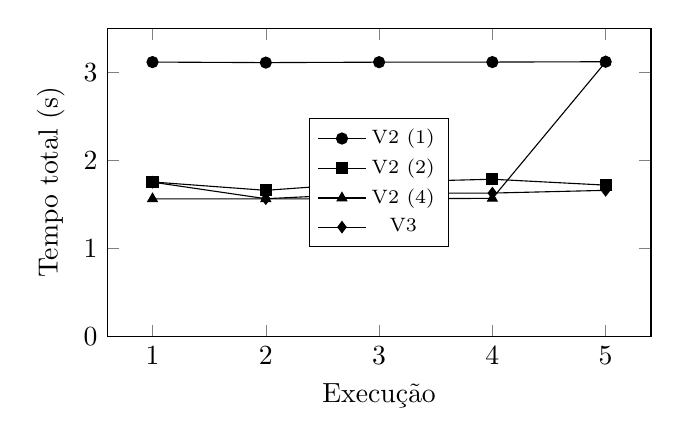
\begin{tikzpicture}
\begin{axis}[width=0.7\textwidth, height=5.5cm, xlabel={Execução}, ylabel={Tempo total (s)}, xtick={1,...,5}, ymin=0, ymax=3.5, legend style={font=\scriptsize, at={(0.5,0.5)}, anchor=center}, mark size=2pt]
\addplot[mark=*] coordinates {(1,3.116)(2,3.110)(3,3.115)(4,3.116)(5,3.120)};
\addplot[mark=square*] coordinates {(1,1.756)(2,1.661)(3,1.754)(4,1.787)(5,1.720)};
\addplot[mark=triangle*] coordinates {(1,1.564)(2,1.565)(3,1.565)(4,1.570)(5,3.117)};
\addplot[mark=diamond*] coordinates {(1,1.754)(2,1.566)(3,1.629)(4,1.630)(5,1.661)};
\legend{V2 (1), V2 (2), V2 (4), V3}
\end{axis}
\end{tikzpicture}
\caption{Tempo total em cada execução. A execução 5 da V2 (limite 4) caiu no regime serializado.}
\end{figure}

\subsection{Variabilidade: o ``comboio'' observado}
\label{sec:comboio}
Em 5 execuções, a V2 com limite 4 teve uma de 3,12~s e quatro de 1,56~s. Repetimos o experimento 30 vezes: a V2 com limite 4 caiu no regime serializado (máx.\ comendo $=1$, 3,12~s) em 4 de 30 execuções, e nas outras 26 levou em média 1,57~s. A V2 com limite 2 e a V3 não tiveram nenhuma execução desse tipo nas 30 repetições (médias de 1,72~s e 1,74~s). Na V1, sete das oito execuções que não travaram também levaram 3,1~s. A hipótese é um efeito comboio: os filósofos entram em fila (cada um pega o garfo logo depois de o vizinho soltar) e a execução fica serializada. Não isolamos isso com um experimento específico, então é uma hipótese. Por isso, com poucas execuções, o desvio da V2 (limite 4) é alto, e vale olhar também a mediana (1,56~s).

\subsection{Evidência de Deadlock na V1}
\label{sec:v1}
Em 12 de 20 execuções a V1 travou (as outras 8 completaram: sete em cerca de 3,10~s e uma em 1,56~s). A Figura abaixo mostra a saída do vigia em uma execução que travou, seguida da mensagem do runtime do Go:

\begin{figure}[H]
\centering
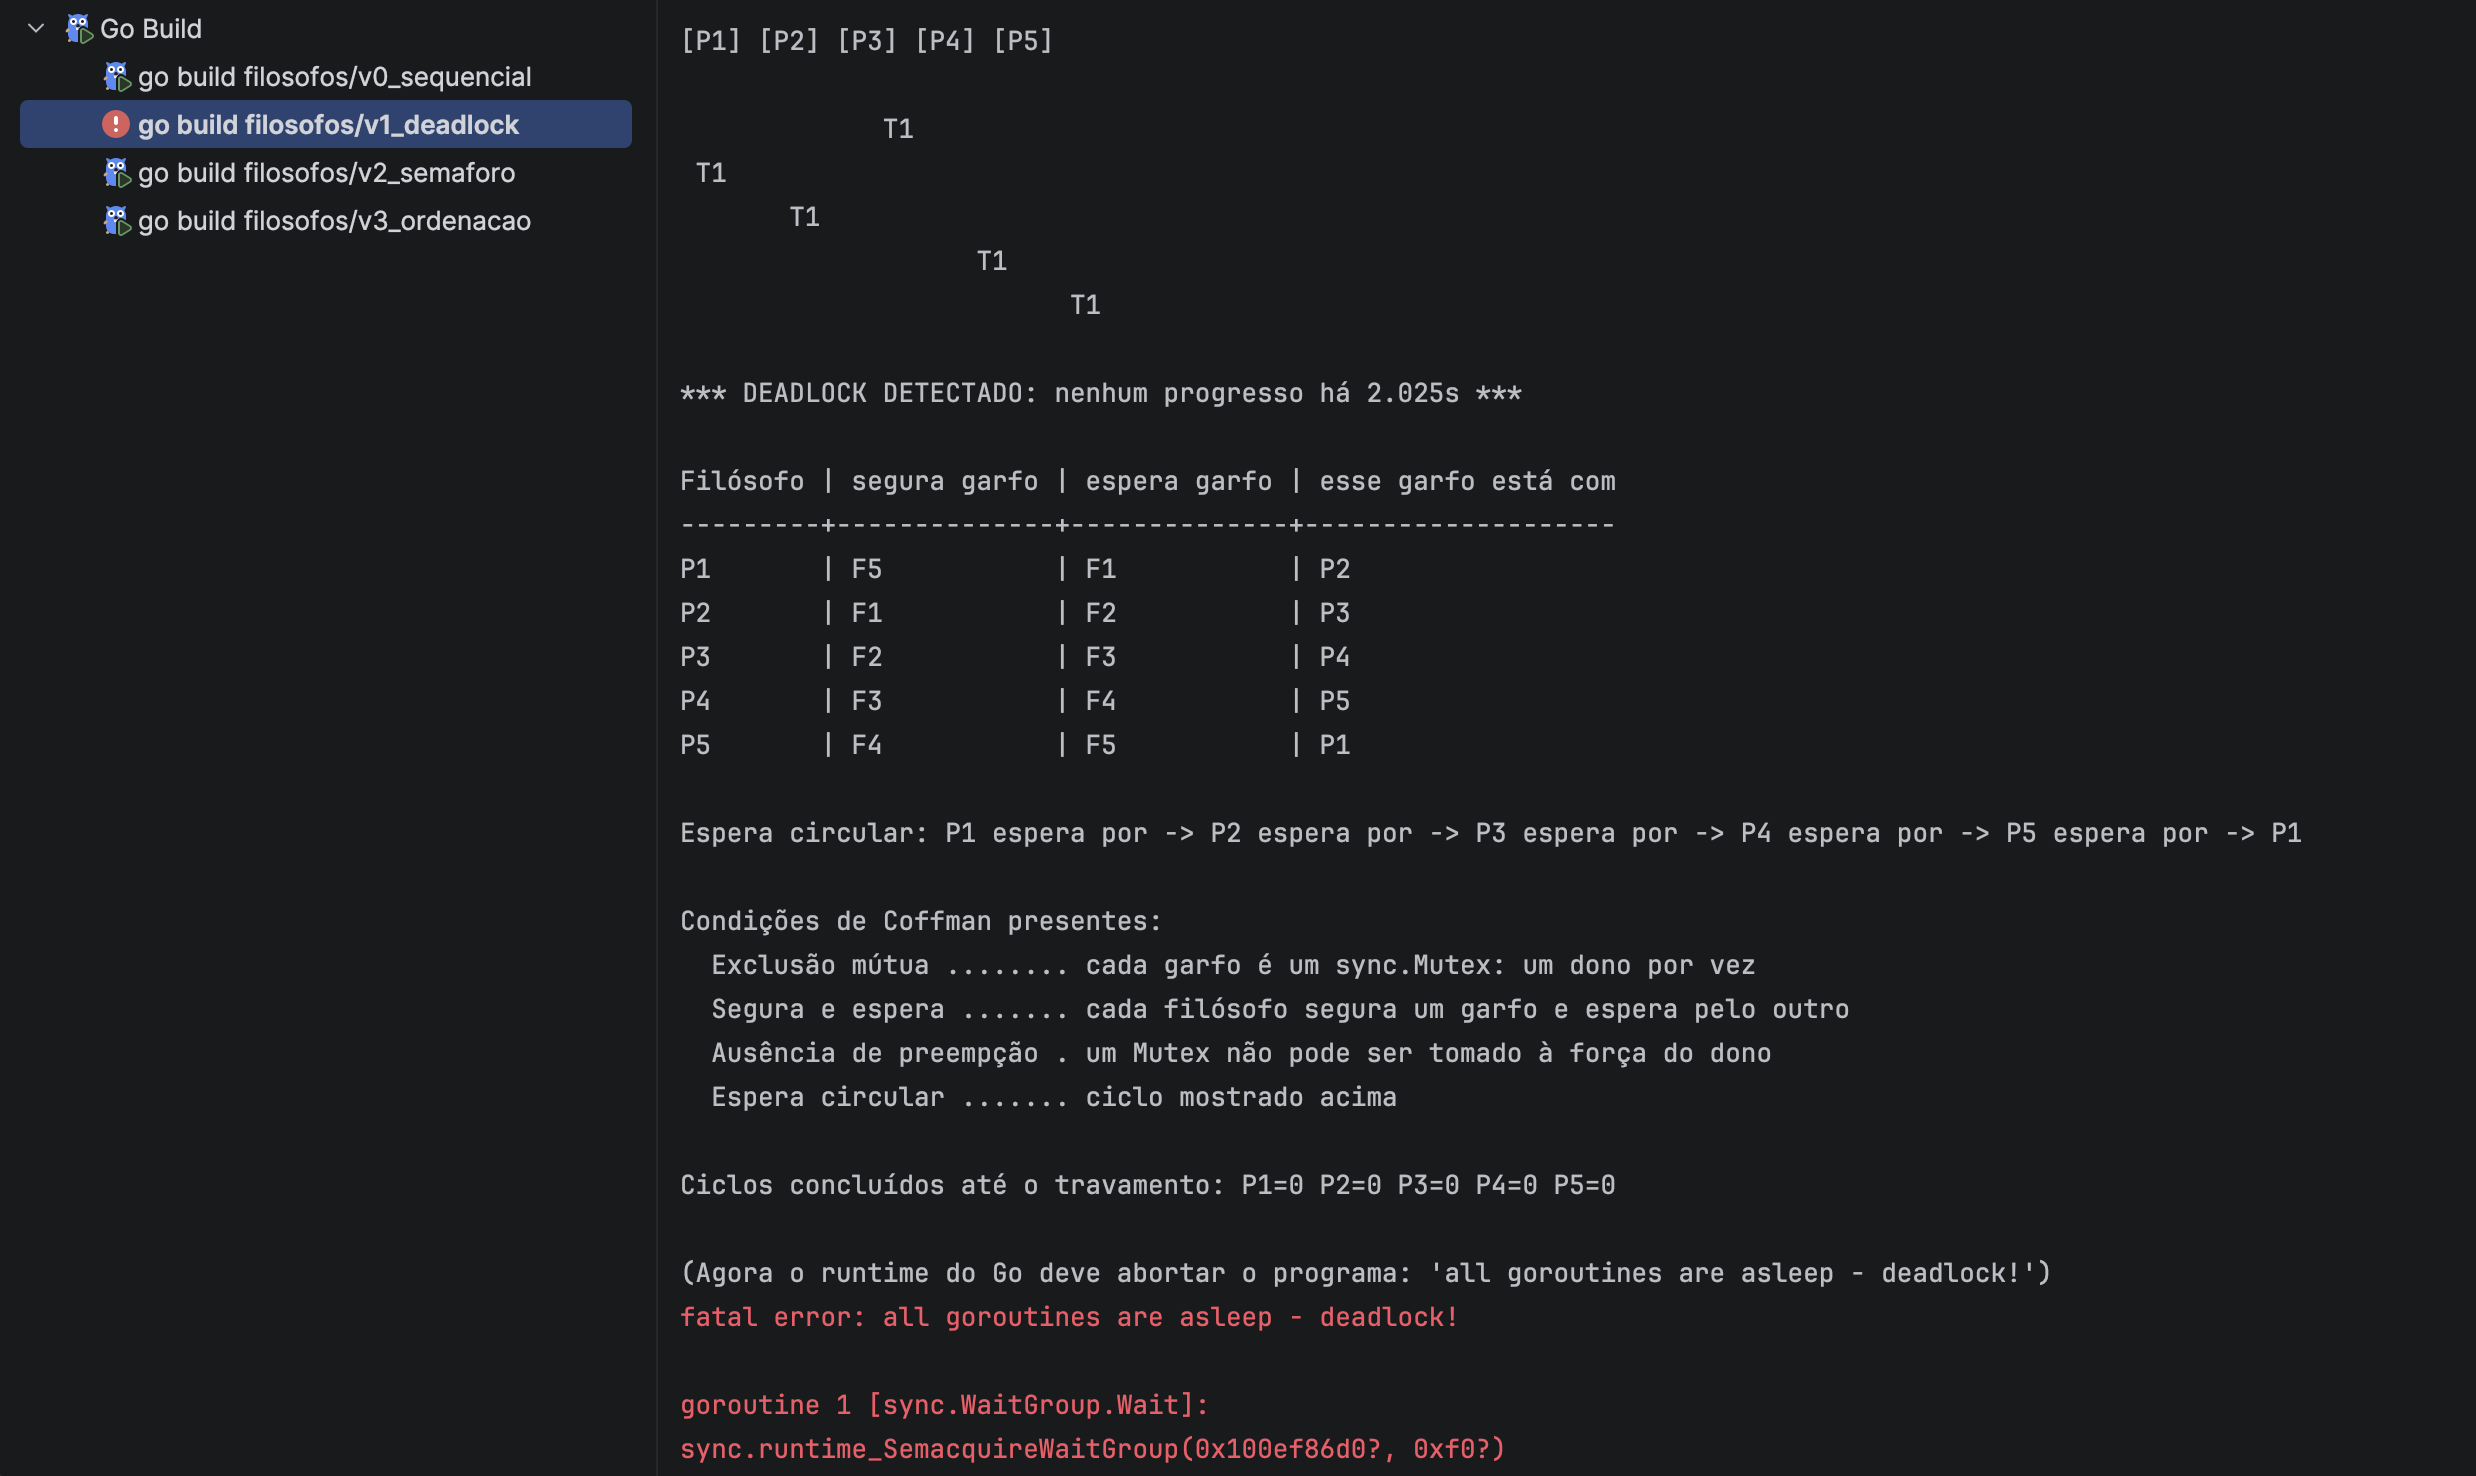
\includegraphics[width=\textwidth]{v1-deadlock.png}
\caption{Saída da V1 em deadlock: tabela de quem segura e espera cada garfo, espera circular, condições de Coffman e a mensagem do runtime do Go.}
\end{figure}

O estado capturado tem a forma esperada: P1 segura F5 e espera F1 (com P2), P2 segura F1 e espera F2 (com P3), P3 segura F2 e espera F3 (com P4), P4 segura F3 e espera F4 (com P5), P5 segura F4 e espera F5 (com P1). Todas as goroutines ficam em \texttt{sync.Mutex.Lock}, e ninguém terminou nenhum ciclo. As quatro condições de Coffman estão presentes: exclusão mútua (cada garfo é um \texttt{Mutex}), posse e espera (cada filósofo segura um garfo e pede o outro), ausência de preempção (um \texttt{Mutex} não é tomado à força) e espera circular (o ciclo acima).

%% ------------------------------------------------------------------
\section{Análise dos Resultados}

O funcionamento de cada solução, os mecanismos de sincronização e sua implementação em Go estão descritos na Seção~2. Em resumo, a V0 não sincroniza nada, a V1 usa um \texttt{sync.Mutex} por garfo, a V2 acrescenta um semáforo feito com canal com buffer (o garçom) e a V3 usa só \texttt{Mutex} com uma ordem global de aquisição. Esta seção usa as métricas da Seção~4 para explicar as diferenças entre elas.

\subsection{Deadlock na V1 e como V2 e V3 o evitam}
A V1 trava porque as quatro condições de Coffman estão presentes. Há exclusão mútua, pois o \texttt{Mutex} tem um dono por vez. Há posse e espera, pois cada filósofo segura o garfo esquerdo e espera o direito. Não há preempção, pois o \texttt{Mutex} não pode ser tomado do dono. E há espera circular: se os cinco pegam o garfo esquerdo antes de qualquer um pegar o direito, P1 espera P2, que espera P3, e assim por diante até P5 esperar P1. Ninguém solta o garfo que tem, então ninguém progride. A flag \texttt{-atraso} aumenta a janela em que isso acontece e, com \texttt{-jitter 0}, o deadlock ocorre sempre. Com o pensar sorteado, a V1 travou em 12 de 20 execuções, sem nenhum ciclo concluído (Figura da Seção~4.4).

A V2 e a V3 quebram a espera circular de formas diferentes. Na V2 o garçom deixa no máximo $N-1$ filósofos disputando os garfos. Como $N-1$ filósofos disputam $N$ garfos, pelo menos um consegue os dois, come e libera, e o ciclo completo de esperas nunca se forma. Na V3 a ordem global faz com que quem espera pelo garfo $k$ já segure um garfo de número menor, então qualquer cadeia de esperas é estritamente crescente e não fecha ciclo. Na prática, P5 segura F4 e espera F5, mas P1 nunca segura F5 esperando F1, porque pega F1 primeiro.

\subsection{Starvation}
Evitar deadlock não elimina starvation. Na V2 a fila do canal é atendida em ordem de chegada, então a espera pelo garçom é limitada. Nos \texttt{Mutex}, o Go entra em modo de justiça depois de 1~ms de espera, o que limita o risco na prática. Na V3 o algoritmo não garante que um filósofo não seja ultrapassado repetidamente pelos vizinhos, então a starvation é teoricamente possível. Nos experimentos ela não foi observada: em todas as execuções de V2 e V3 os cinco filósofos concluíram os 20 ciclos, e a maior espera foi de 124~ms, cerca de quatro refeições de 30~ms, longe de um adiamento indefinido.

\subsection{Tempo total e tempo de espera}
A tabela abaixo compara as versões com o piso teórico do tempo total, dado pelo número máximo de filósofos comendo ao mesmo tempo (100 refeições de 30~ms divididas entre eles, com o pensar sobreposto).

\begin{center}
\small
\begin{tabular}{lrrrr}
\toprule
Versão & Tempo total (s) & Piso teórico (s) & Espera média (ms) & Máx.\ comendo\\
\midrule
V0 & 5,194 & 5,0 & 0,000 & 1\\
V2 (limite 1) & 3,115 & 3,0 & 100,8 & 1\\
V2 (limite 2) & 1,736 & 1,5 & 32,4 & 2\\
V2 (limite 4) & 1,876 & 1,5 & 40,3 & 2\\
V3 & 1,648 & 1,5 & 25,2 & 2\\
\bottomrule
\end{tabular}
\end{center}

A V0 teve o maior tempo total, 5,194~s, que é a soma de todos os pensar e comer ($100\times50$~ms $=5$~s) mais o custo dos \texttt{Sleep}. Entre as versões concorrentes, a mais lenta foi a V2 com limite 1, com 3,115~s, próximo do piso de 3~s das 100 refeições serializadas. Os demais tempos ficam de 4\% a 17\% acima do piso de 1,5~s por causa da contenção e do escalonamento.

O maior tempo de espera pelos garfos foi o da V2 com limite 1: média de 100,8~ms e máximo de 124,1~ms, pois os cinco fazem fila no garçom e cada um espera cerca de quatro refeições de 30~ms. A V0 teve espera praticamente nula (máximo de 0,003~ms), porque nunca há disputa. A V3 (25,2~ms) e a V2 com limite 2 (32,4~ms) ficaram entre os dois extremos. A maior espera isolada da V3 e da V2 com limite 4 também chegou a 124~ms, em execuções que caíram no regime serializado ou em que um filósofo foi ultrapassado (Seção~\ref{sec:comboio}).

\subsection{Grau de concorrência}
O limite teórico é de 2 filósofos comendo ao mesmo tempo (cinco garfos, dois por filósofo), e ele foi alcançado em todas as versões que o permitem.

\begin{center}
\small
\begin{tabular}{lc}
\toprule
Versão & Máx.\ filósofos comendo juntos\\
\midrule
V0 & 1\\
V1 (execuções que completaram) & 1 (7 execuções) ou 2 (1 execução)\\
V2 (limite 1) & 1\\
V2 (limite 2) & 2\\
V2 (limite 4) & 2 (1 nas execuções serializadas)\\
V3 & 2\\
\bottomrule
\end{tabular}
\end{center}

O tempo total acompanha o grau de concorrência. Com 1 filósofo comendo por vez, o tempo foi de 5,19~s (V0) e 3,12~s (V2 com limite 1). Com 2, ficou entre 1,56 e 1,76~s (V3 e V2 com limites 2 e 4). A V0 é mais lenta que a V2 com limite 1 mesmo tendo o mesmo máximo de 1 comendo, porque na V0 o pensar também é sequencial, enquanto na V2 ele se sobrepõe ao comer dos outros. A execução 5 da V2 com limite 4 ilustra a relação: só teve 1 filósofo comendo e levou 3,12~s, o tempo do regime serializado, apesar de o mecanismo permitir 4 candidatos.

\subsection{Impacto da sincronização excessiva da V2}
Com limite 1, a V2 elimina o paralelismo do comer: apenas um filósofo come por vez, mesmo havendo garfos livres para um não vizinho. Os garfos viram redundantes, já que nunca há disputa por eles. A tabela mostra o efeito de afrouxar o limite, com o tempo do limite 4 tomado das execuções que não caíram no regime serializado.

\begin{center}
\small
\begin{tabular}{lrrr}
\toprule
Versão & Tempo total (s) & Redução vs.\ limite 1 & Espera média (ms)\\
\midrule
V2 (limite 1) & 3,115 & --- & 100,8\\
V2 (limite 2) & 1,736 & 44\% & 32,4\\
V2 (limite 4) & 1,564 & 50\% & 25,2\\
V3 & 1,648 & 47\% & 25,2\\
\bottomrule
\end{tabular}
\end{center}

Passar de 1 para 2 é o que importa; de 2 para 4 quase não há ganho, porque o teto físico já é 2 comendo. Em relação à V3, igualmente livre de deadlock, a V2 com limite 1 é 89\% mais lenta, e esse é o custo da sincronização desnecessária.

\subsection{Mais sincronização significa melhor desempenho?}
Não. A V2 com limite 1 sincroniza mais que a V3, porque protege por inteiro uma região que não precisava ser protegida por inteiro, e perdeu: 3,115~s e espera média de 100,8~ms, contra 1,648~s e 25,2~ms da V3. A V2 com limite 2 (1,736~s) e a V3 ficaram próximas, e a V3 não precisa de coordenador central. No outro extremo, a V1 tem sincronização mínima e trava. O desempenho depende de usar a sincronização só onde há conflito real, que aqui é a disputa pelo mesmo garfo.

%% ------------------------------------------------------------------
\section{Conclusões}
A V1 mostra que exclusão mútua simples por garfo basta para travar: com cada filósofo pegando primeiro o garfo esquerdo, a espera circular se formou em 12 de 20 execuções, sem nenhum ciclo concluído. A V2 e a V3 evitam o problema por mecanismos diferentes (limitar candidatos a $N-1$ ou impor ordem global), mas com custos de desempenho muito diferentes: com limite 1 o garçom serializa o comer (3,12~s, espera média de 100,8~ms), enquanto a V3 chega a 1,65~s com espera média de 25,2~ms e dois filósofos comendo juntos, o máximo possível com cinco garfos. O tempo total acompanhou o máximo de filósofos comendo (1 $\rightarrow$ 3,1 a 5,2~s; 2 $\rightarrow$ 1,6 a 1,8~s), e mais sincronização não foi sinônimo de melhor desempenho. A melhor solução, em tempo médio e sem coordenador central, foi a V3. Ressalvas: a V3 não garante ausência de starvation (não foi observada), e a variabilidade da V2 com limite 4 mostra que poucas execuções podem esconder regimes diferentes.

%% ------------------------------------------------------------------
\section*{Repositório}
Código-fonte completo: \url{https://github.com/lpmilitao/JantarDosFilosofos}

% \bibliographystyle{plain}
% \bibliography{referencias}

\end{document}
